\chapter{PROCEDURE} \label{ch:procedure}
Each team is provided with 4 column cards such as \texttt{TO DO}, \texttt{DOING}, \texttt{TEST}, \texttt{DONE} and 9 task cards (actually colorful sticky notes). Team members selected task according to their choice. The first step is to do independent works such as "Data Collection". I was assigned task 4 and 6 which were to collect data of ages and favorite food of all team members.
\begin{figure}[H]
    \centering
    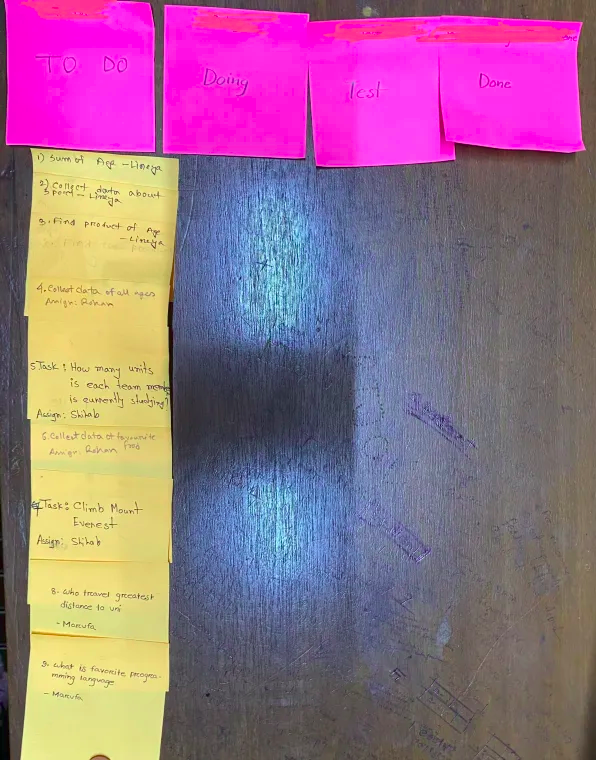
\includegraphics[width=0.5\linewidth]{phase-1.png}
    \caption{Phase 1}
    \label{fig:placeholder}
\end{figure}

Then 6 tasks were shifted to \texttt{DOING} section, basically the independent ones. The remaining tasks which were dependent stayed in the first column.

\begin{figure}[H]
    \centering
    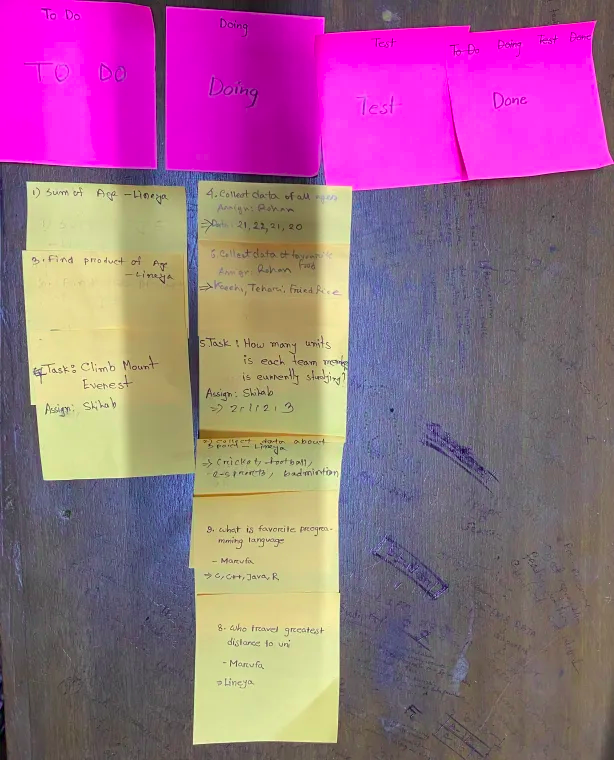
\includegraphics[width=0.5\linewidth]{figures/phase-2.png}
    \caption{Phase 2}
    \label{fig:placeholder}
\end{figure}

After that 5 tasks were done without testing because most of them didn't requite that, they were basically data collection, non-calculation tasks. And one task (distance) was in the testing phase.

\begin{figure}[H]
    \centering
    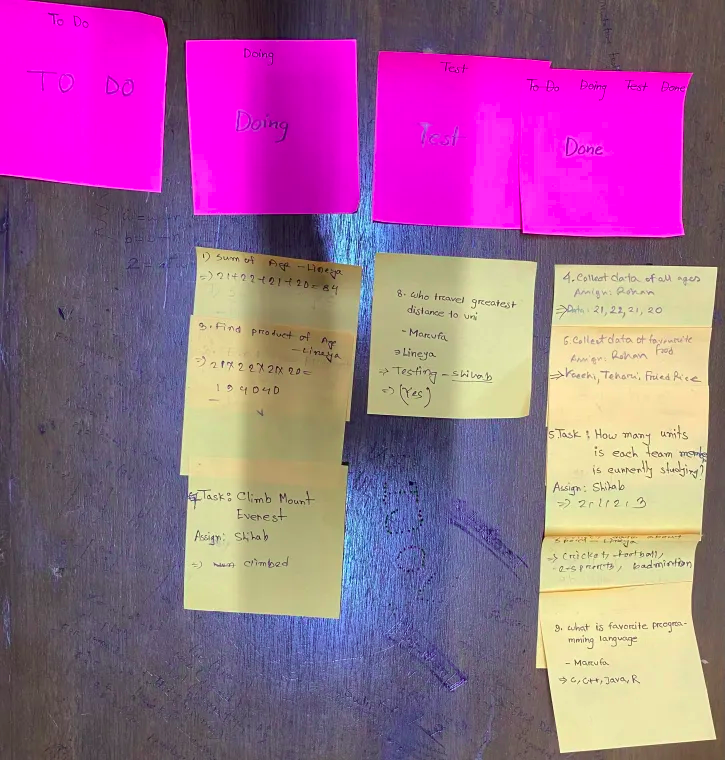
\includegraphics[width=0.5\linewidth]{figures/phase-3.png}
    \caption{Phase 3}
    \label{fig:placeholder}
\end{figure}

And finally all the tasks passed the testing column. 'Climbing Mount Everest' remained in the doing column because it was impossible for us to climb mountain in the computer lab. So, it got stucked in the  \texttt{DOING}.

\begin{figure}[H]
    \centering
    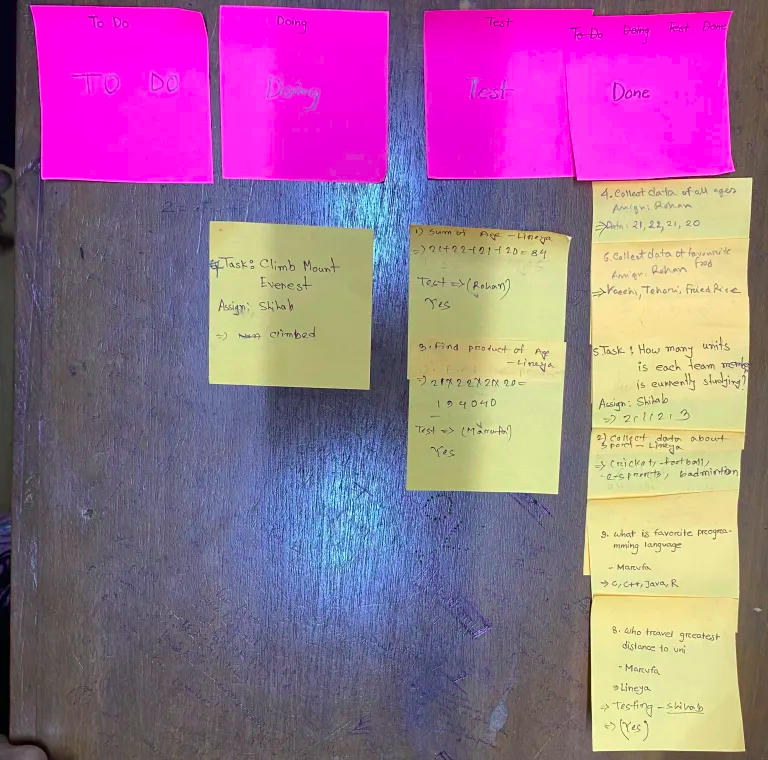
\includegraphics[width=0.5\linewidth]{figures/phase-4.png}
    \caption{Phase 4}
    \label{fig:placeholder}
\end{figure}
\begin{figure}[H]
    \centering
    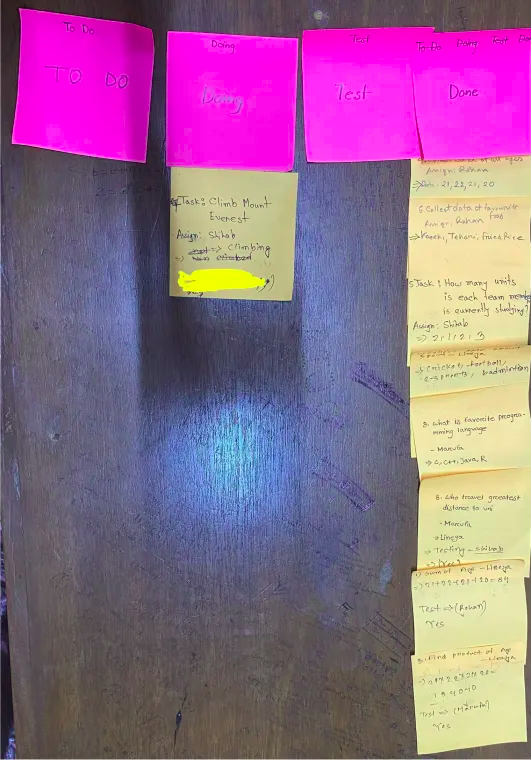
\includegraphics[width=0.5\linewidth]{figures/phase-5.png}
    \caption{Phase 5}
    \label{fig:placeholder}
\end{figure}